%Type of Document
\documentclass[a4paper, 12pt]{report}

%Load Pre-ambles
\usepackage{../../Environment/Packages}
\usepackage{../../Environment/Conventions}
\usepackage{../../Environment/Hyahoos}

\begin{document}

\begin{center}
%Seperator
%Seperator
%Seperator
%Seperator
%Seperator
%Seperator
\chapter{Rigid Body Kinematics}
\begin{comment}
\end{comment}
%Seperator
%Seperator
%Seperator
%Seperator
%Seperator
\section{Direction Cosine Matrix}
\begin{comment}
\end{comment}
The dot product can be thought as some form of projection of one vector onto another vector. Consider the dot product of two vectors $\b{a}$ and $\b{b}$. Based on the definition of dot product,
$$\b{a}\d\b{b} = |a||b|\cos\t$$
wherein $\t$ is the angle between the vectors $\b{a}$ and $\b{b}$. Let an arbitrary vector $\b{r}$ be represented in basis vectors $\h{i}$, $\h{j}$, and $\h{k}$. Let these basis vectors be of mangitude $1$. Let another set of basis vectors of magnitude $1$ be defined as $\h{i}'$, $\h{j}'$, and $\h{k}'$. The arbitrary vector $\b{r}$ could be expressed as a linear combination of these basis vectors,
$$\b{r} = x\h{i} + y\h{j} + z\h{k} = x'\h{i}' + y'\h{j}' + z'\h{k}'$$

The vector component $\b{r}$ in the $\h{i}'$ direction is the summation of all the weighted basis vector components on the $\h{i}'$ direction. Since it was established earlier that this would mean taking the dot product,
$$x' = x(\h{i}\d\h{i}') + y(\h{j}\d\h{i}') + z(\h{k}\d\h{i}')$$
Let $\t_{fg'}$ represent the angle between the $f$ axis and the $g'$ axis,
$$\h{i}\d\h{i}' = |\h{i}||\h{i}'|\cos\t_{ii'} \quad,\quad \h{j}\d\h{i}' = |\h{j}||\h{i}'|\cos\t_{ji'} \quad,\quad \h{k}\d\h{i}' = |\h{k}||\h{i}'|\cos\t_{ki'}$$
Using the earlier assumption that the magnitude of the basis vectors are all $1$,
$$\h{i}\d\h{i}' = \cos\t_{ii'} \quad,\quad \h{j}\d\h{i}' = \cos\t_{ji'} \quad,\quad \h{k}\d\h{i}' = \cos\t_{ki'}$$
Substituting the basis vector projections,
$$x' = x\cos\t_{ii'} + y\cos\t_{ji'} + z\cos\t_{ki'}$$

Repeating similar operations for the $\h{j}'$ direction,
$$y' = x(\h{i}\d\h{j}') + y(\h{j}\d\h{j}') + z(\h{k}\d\h{j}')$$
$$\h{i}\d\h{j}' = |\h{i}||\h{j}'|\cos\t_{ij'} \quad,\quad \h{j}\d\h{j}' = |\h{j}||\h{j}'|\cos\t_{jj'} \quad,\quad \h{k}\d\h{j}' = |\h{k}||\h{j}'|\cos\t_{kj'}$$
Using the earlier assumption that the magnitude of the basis vectors are all $1$,
$$\h{i}\d\h{j}' = \cos\t_{ij'} \quad,\quad \h{j}\d\h{j}' = \cos\t_{jj'} \quad,\quad \h{k}\d\h{j}' = \cos\t_{kj'}$$
Substituting the basis vector projections,
$$y' = x\cos\t_{ij'} + y\cos\t_{jj'} + z\cos\t_{kj'}$$

Repeating similar operations for the $\h{k}'$ direction,
$$z' = x(\h{i}\d\h{k}') + y(\h{j}\d\h{k}') + z(\h{k}\d\h{k}')$$
$$\h{i}\d\h{k}' = |\h{i}||\h{k}'|\cos\t_{ik'} \quad,\quad \h{j}\d\h{k}' = |\h{j}||\h{k}'|\cos\t_{jk'} \quad,\quad \h{k}\d\h{k}' = |\h{k}||\h{k}'|\cos\t_{kk'}$$
Using the earlier assumption that the magnitude of the basis vectors are all $1$,
$$\h{i}\d\h{k}' = \cos\t_{ik'} \quad,\quad \h{j}\d\h{k}' = \cos\t_{jk'} \quad,\quad \h{k}\d\h{k}' = \cos\t_{kk'}$$
Substituting the basis vector projections,
$$z' = x\cos\t_{ik'} + y\cos\t_{jk'} + z\cos\t_{kk'}$$

Collecting the various expressions together,
$$x' = x\cos\t_{ii'} + y\cos\t_{ji'} + z\cos\t_{ki'}$$
$$y' = x\cos\t_{ij'} + y\cos\t_{jj'} + z\cos\t_{kj'}$$
$$z' = x\cos\t_{ik'} + y\cos\t_{jk'} + z\cos\t_{kk'}$$

Re-arranging the expressions into matrix form,
$$\begin{bmatrix}
x' \\ y' \\ z'
\end{bmatrix} = \begin{bmatrix}
\cos\t_{ii'} && \cos\t_{ji'} && \cos\t_{ki'} \\
\cos\t_{ij'} && \cos\t_{jj'} && \cos\t_{kj'} \\
\cos\t_{ik'} && \cos\t_{jk'} && \cos\t_{kk'}
\end{bmatrix}\begin{bmatrix}
x \\ y \\ z
\end{bmatrix}$$
Hence, based on the problem definition,
$$\b{r}' = \begin{bmatrix}
x' \\ y' \\ z'
\end{bmatrix} \quad,\quad \b{r} = \begin{bmatrix}
x \\ y \\ z
\end{bmatrix} \quad,\quad l = \begin{bmatrix}
\cos\t_{ii'} && \cos\t_{ji'} && \cos\t_{ki'} \\
\cos\t_{ij'} && \cos\t_{jj'} && \cos\t_{kj'} \\
\cos\t_{ik'} && \cos\t_{jk'} && \cos\t_{kk'}
\end{bmatrix}$$
$$\b{r}' = l \b{r}$$
The figure below shows some of the angles referenced in the $l$ matrix,
%\\~\\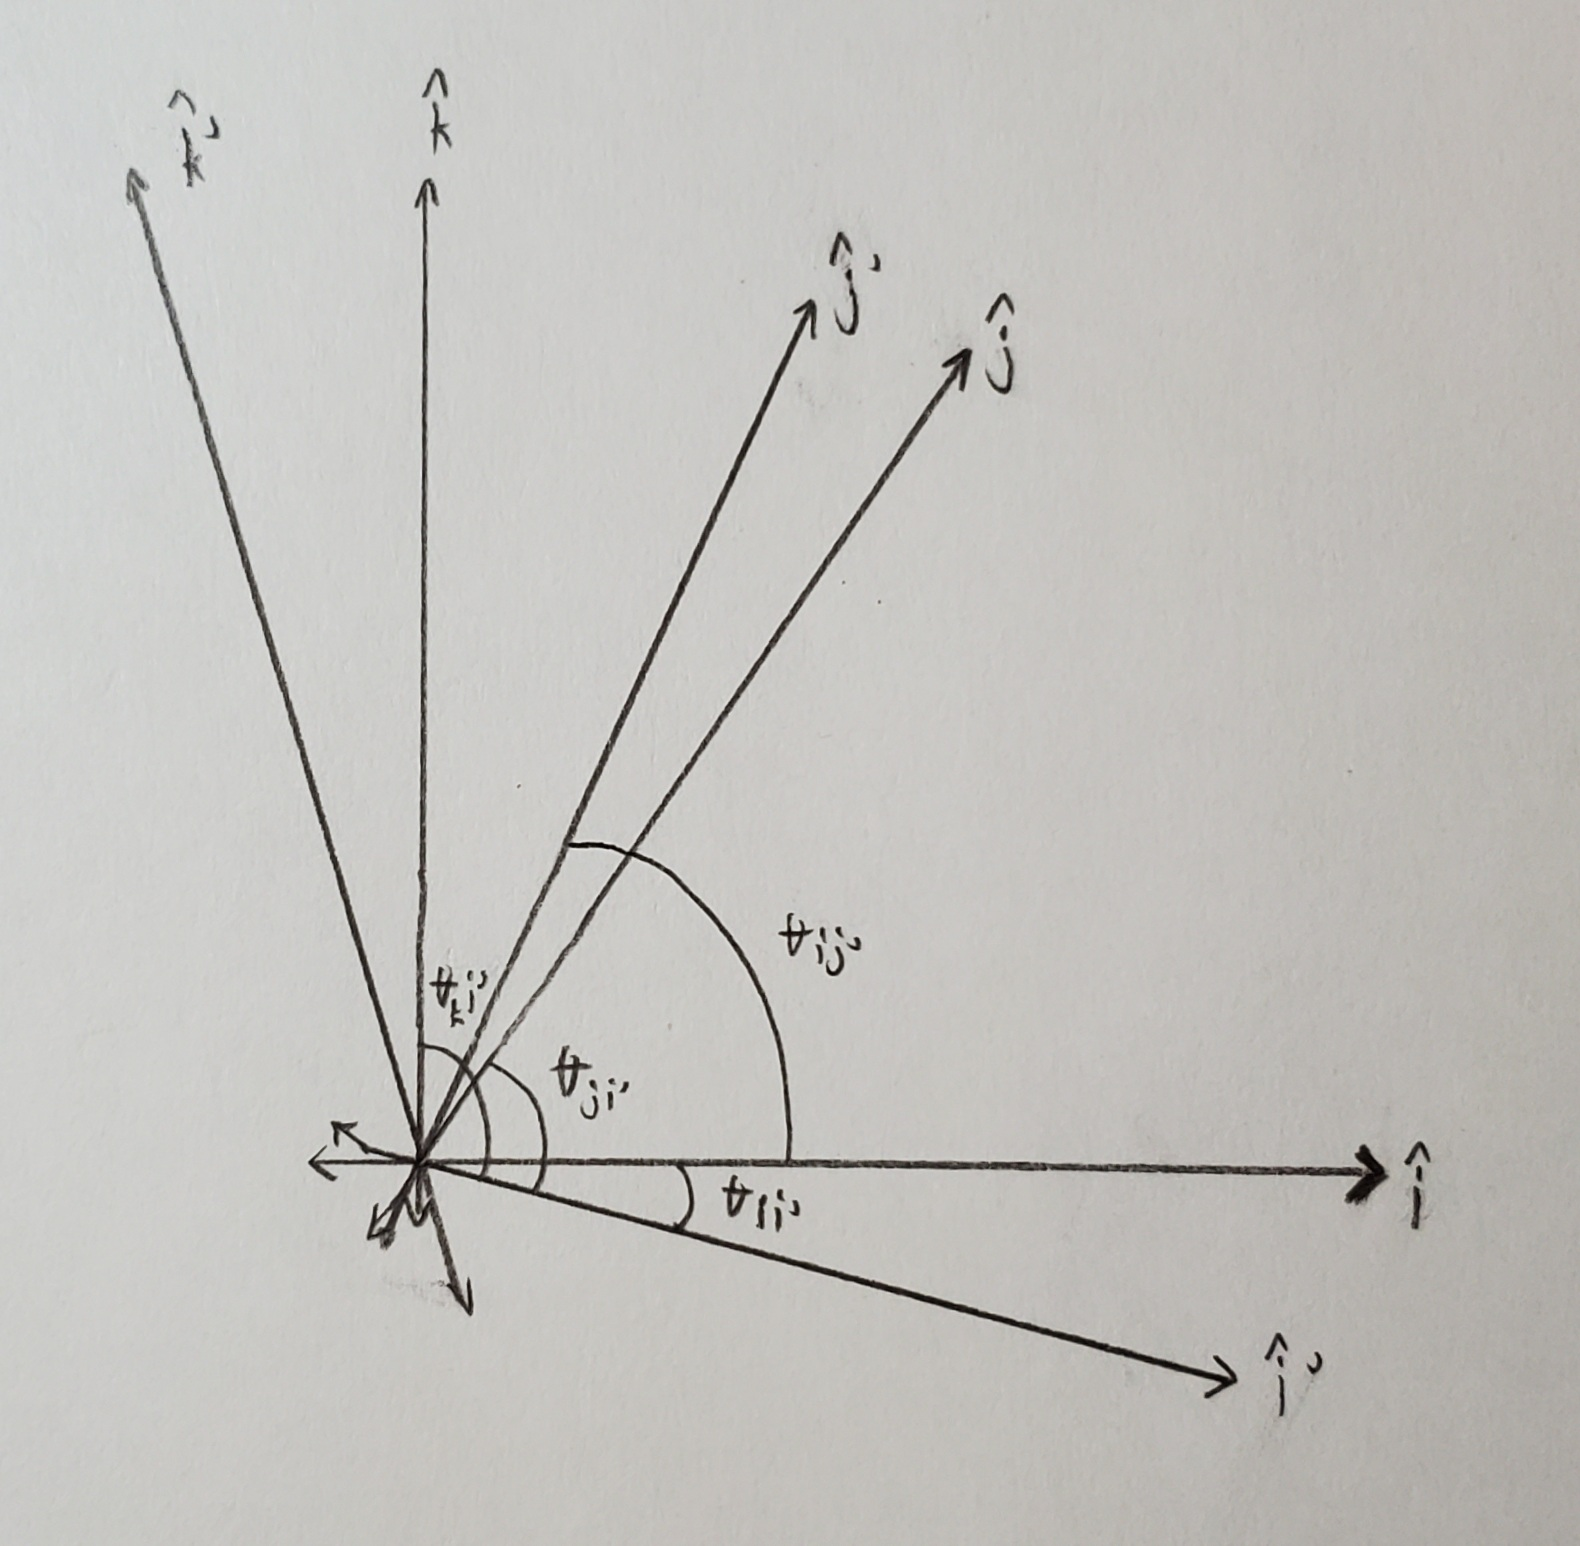
\includegraphics[scale=\sizes]{Bajing_Terbang}
%Seperator
%Seperator
%Seperator
%Seperator
%Seperator
\end{center}

\end{document}
